
\subsection{Mahne, Baglin, Collins et al. 2004 (ELETTRA)}
\label{sec:Mahne}
This paper~\cite{mahne} covers only the photon reflectivity distributions, these were measured at ELETTRA, Italy.

\subsubsection{Experiment setup}
The experiment discussed in this paper is based on measured photons instead of electrons, see Fig.~\ref{fig:exp_mahne}.
Copper samples with and without sawtooth were irradiated with synchrotron light between 8 and 200~eV.
The reflectivity of the samples were measured in different directions.
The electron yields however could not be recorded.

\begin{figure}[tbh]
    \centering
    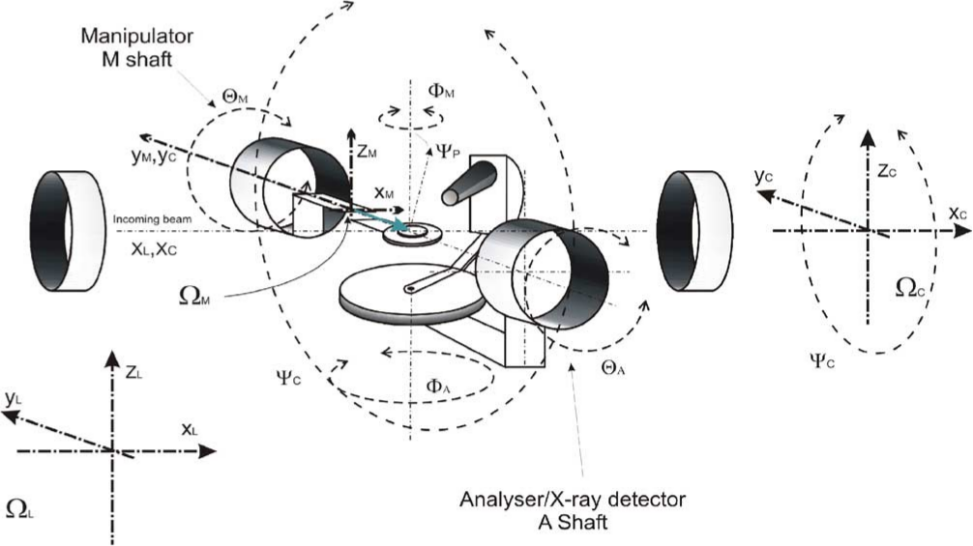
\includegraphics[width=0.8\textwidth]{../ss/experiment_mahne.png}
    \caption{The experiment setup from Sec.~\ref{sec:Mahne}.}
    \label{fig:exp_mahne}
\end{figure}


\subsubsection{Results}

The main results are listed in Fig.~\ref{fig:mahne}.
First, the reflectivity depending on the angle is shown for synchrotron radiation with a critical energy of 44~eV, similar to the previously discussed paper from Baglin et al.
The difference is that not only the reflectivity in forward direction was measured, but in all directions.
Figure~\ref{fig:mahne} (bottom) specifies the total reflectivity.
In case of the sawtooth, reflectivity increases from 1.8\% to 10\%.

Furthermore, it was found that the reflectivity depends on the photon energy.
This means that also the spectrum of reflected photons is different from the original one.


\subsubsection{Open questions}
Some inconsistencies exist.
\begin{itemize}
    \item The Baglin paper from Sec.~\ref{sec:Baglin} measured reflectivity as 1.8\% for the sawtooth sample, whereas the forward scattering in this paper alone amounts to 4\%.
    \item Furthermore, it is unclear how the 2\% diffused photons are obtained from a white light spectrum.
        In Fig.~\ref{fig:mahne} (right), the amount of diffused photons never reaches 2\% for any photon energy.
        %Certainly, the 2\% cannot be reached for a spectrum of photons, either.
        This discrepancy is not commented in the paper.
    \item The photon flux is not stated, photon scrubbing is not mentioned.
\end{itemize}


\begin{figure}[tbh]
    \centering
    \begin{minipage}[c]{0.47\textwidth}
        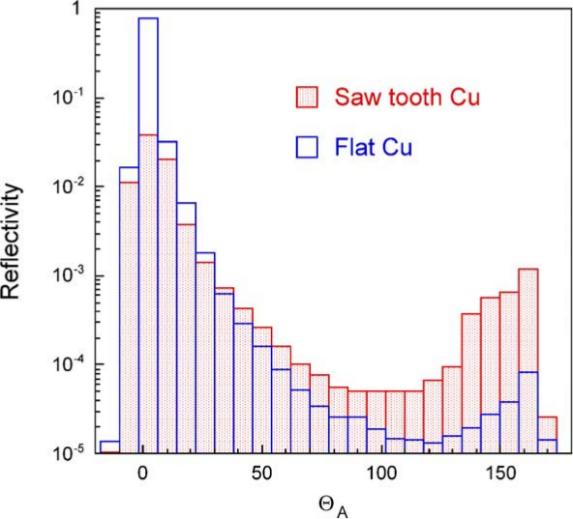
\includegraphics[width=\textwidth]{../ss/mahne_refl.png}
    \end{minipage}
    \hspace{0.5cm}
    \begin{minipage}[c]{0.47\textwidth}
        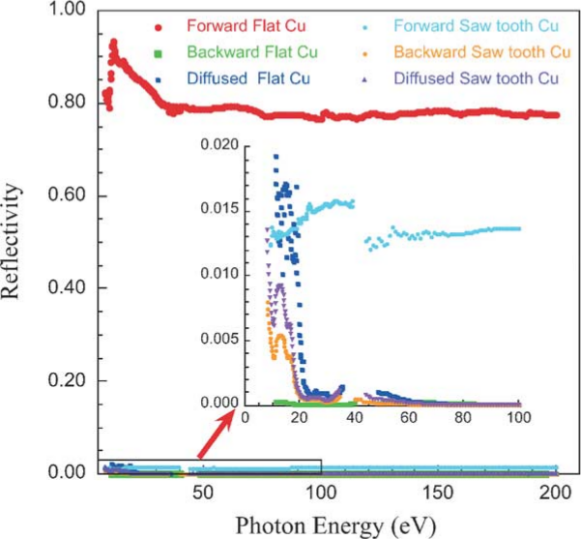
\includegraphics[width=\textwidth]{../ss/mahne_yield.png}
    \end{minipage}

    \begin{minipage}[c]{0.48\textwidth}
        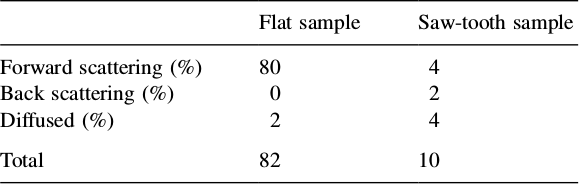
\includegraphics[width=\textwidth]{../ss/mahne_table.png}
    \end{minipage}
    \caption{
        Left: Measured reflectivity of Cu samples for different angles after grazing incidence.
        \\
        Right: Measured electron yield of Cu samples.
        \\
        Bottom: Summary of reflectivities for a LHC-type spectrum from the paper presented in Sec.~\ref{sec:Mahne}.
    }
    \label{fig:mahne}

\end{figure}



